\documentclass[10pt]{article}

\usepackage{amsfonts}
\usepackage{amsmath}
\usepackage{geometry}
\usepackage[dvipsnames]{xcolor}
\usepackage{graphicx}
\usepackage{subcaption}
\usepackage{listings}

\definecolor{codegreen}{rgb}{0,0.6,0}
\definecolor{codegray}{rgb}{0.5,0.5,0.5}
\definecolor{codepurple}{rgb}{0.58,0,0.82}
\definecolor{backcolour}{rgb}{0.95,0.95,0.92}
 
\lstdefinestyle{mystyle}{
    emph={init, RK, initialize},
    emphstyle=\color{PineGreen},
    commentstyle=\color{blue},
    keywordstyle={\color{BrickRed}\bfseries},
    numberstyle=\color{codegray},
    stringstyle=\color{codepurple},
    breakatwhitespace=false,         
    breaklines=true,                 
    captionpos=b,                    
    keepspaces=true,                 
    numbers=left,                    
    numbersep=5pt,                  
    showspaces=false,                
    showstringspaces=false,
    showtabs=false              
}

\title{Modeling Stars: \\ Two Method Comparison and Analysis}
\author{Najla Alahmadi, Michael Cock, Rebecca Halloran, Brady Metherall, Hector Robinson}

\newgeometry{margin=1in}
\setlength\parindent{0pt}

\begin{document}
\maketitle

\lstset{style=mystyle}
\section{Introduction}
In this project, we modelled a spherically symmetric, static star by numerically integrating the four stellar equations. We started by doing this for a star that had the same core conditions as the sun, and then changed the intial conditions to determine final values for many other stars. We had to be careful with the initial conditions we used to ensure that the temperature and pressure went to zero at the surface. The initial conditions were valid as long as the temperature decayed as expected. Using the results, we can plot the relation between luminosity and temperature of the stars to create an Hertzpring-Russell Diagram (HR diagram). We created code that would be able to take a stars composition, mass and some initial conditions to determine surface temperature, surface luminosity and surface radius so we can plot the surface luminosity versus the surface temperature or an HR diagram. Before we get there, lets talk about our program that will numerically integrate one star. \\

\section{Method}
To perform the calculations we started from the core and integrated outward using the fourth order Runge-Kutta method. We specified a core pressure, core temperature, core density, and composition of the star. From there, the outward integration calculates total mass, luminosity, pressure, and temperature at every other radius. The integration stops when the boundary conditions are met, that is, the pressure or temperature goes to zero. Once this point is reached it means we are at the surface, and have our final values. Figure \ref{fig:code} shows our main code that ran the simulations. Once we have this working for one star using the suns core conditions, we can extend the code to work for many stars. The way to do this is simply by changing the initial conditions. All of our stars had the same compositions; what we changed was the initial core temperature and pressure. We multiplied the core temperature and pressure by a value and used many different values to get different stars.\\

\begin{figure}[htbp]

 \begin{subfigure}{\textwidth}
  \lstinputlisting[language=Python, firstnumber=8, firstline=8, lastline=24]{../solver/main.py}
  \lstinputlisting[language=Python, firstnumber=35, firstline=35, lastline=35]{../solver/main.py}
  \lstinputlisting[language=Python, firstnumber=43, firstline=43, lastline=43]{../solver/main.py}
  \lstinputlisting[language=Python, firstnumber=77, firstline=77, lastline=78]{../solver/main.py}
  \caption{First \emph{main.py} calls \emph{initialize.init} to define our constants, then the core conditions are specified. We then open our data file, run our Runge-Kutta method, and then print the results to the data file.}
 \end{subfigure}
 \caption{main method of the code.}
 \label{fig:code}
\end{figure}

\begin{figure}[p]
\begin{centering}
 \begin{subfigure}{\textwidth}
  % GNUPLOT: LaTeX picture with Postscript
\begingroup
  \makeatletter
  \providecommand\color[2][]{%
    \GenericError{(gnuplot) \space\space\space\@spaces}{%
      Package color not loaded in conjunction with
      terminal option `colourtext'%
    }{See the gnuplot documentation for explanation.%
    }{Either use 'blacktext' in gnuplot or load the package
      color.sty in LaTeX.}%
    \renewcommand\color[2][]{}%
  }%
  \providecommand\includegraphics[2][]{%
    \GenericError{(gnuplot) \space\space\space\@spaces}{%
      Package graphicx or graphics not loaded%
    }{See the gnuplot documentation for explanation.%
    }{The gnuplot epslatex terminal needs graphicx.sty or graphics.sty.}%
    \renewcommand\includegraphics[2][]{}%
  }%
  \providecommand\rotatebox[2]{#2}%
  \@ifundefined{ifGPcolor}{%
    \newif\ifGPcolor
    \GPcolortrue
  }{}%
  \@ifundefined{ifGPblacktext}{%
    \newif\ifGPblacktext
    \GPblacktexttrue
  }{}%
  % define a \g@addto@macro without @ in the name:
  \let\gplgaddtomacro\g@addto@macro
  % define empty templates for all commands taking text:
  \gdef\gplbacktext{}%
  \gdef\gplfronttext{}%
  \makeatother
  \ifGPblacktext
    % no textcolor at all
    \def\colorrgb#1{}%
    \def\colorgray#1{}%
  \else
    % gray or color?
    \ifGPcolor
      \def\colorrgb#1{\color[rgb]{#1}}%
      \def\colorgray#1{\color[gray]{#1}}%
      \expandafter\def\csname LTw\endcsname{\color{white}}%
      \expandafter\def\csname LTb\endcsname{\color{black}}%
      \expandafter\def\csname LTa\endcsname{\color{black}}%
      \expandafter\def\csname LT0\endcsname{\color[rgb]{1,0,0}}%
      \expandafter\def\csname LT1\endcsname{\color[rgb]{0,1,0}}%
      \expandafter\def\csname LT2\endcsname{\color[rgb]{0,0,1}}%
      \expandafter\def\csname LT3\endcsname{\color[rgb]{1,0,1}}%
      \expandafter\def\csname LT4\endcsname{\color[rgb]{0,1,1}}%
      \expandafter\def\csname LT5\endcsname{\color[rgb]{1,1,0}}%
      \expandafter\def\csname LT6\endcsname{\color[rgb]{0,0,0}}%
      \expandafter\def\csname LT7\endcsname{\color[rgb]{1,0.3,0}}%
      \expandafter\def\csname LT8\endcsname{\color[rgb]{0.5,0.5,0.5}}%
    \else
      % gray
      \def\colorrgb#1{\color{black}}%
      \def\colorgray#1{\color[gray]{#1}}%
      \expandafter\def\csname LTw\endcsname{\color{white}}%
      \expandafter\def\csname LTb\endcsname{\color{black}}%
      \expandafter\def\csname LTa\endcsname{\color{black}}%
      \expandafter\def\csname LT0\endcsname{\color{black}}%
      \expandafter\def\csname LT1\endcsname{\color{black}}%
      \expandafter\def\csname LT2\endcsname{\color{black}}%
      \expandafter\def\csname LT3\endcsname{\color{black}}%
      \expandafter\def\csname LT4\endcsname{\color{black}}%
      \expandafter\def\csname LT5\endcsname{\color{black}}%
      \expandafter\def\csname LT6\endcsname{\color{black}}%
      \expandafter\def\csname LT7\endcsname{\color{black}}%
      \expandafter\def\csname LT8\endcsname{\color{black}}%
    \fi
  \fi
    \setlength{\unitlength}{0.0500bp}%
    \ifx\gptboxheight\undefined%
      \newlength{\gptboxheight}%
      \newlength{\gptboxwidth}%
      \newsavebox{\gptboxtext}%
    \fi%
    \setlength{\fboxrule}{0.5pt}%
    \setlength{\fboxsep}{1pt}%
\begin{picture}(8640.00,2880.00)%
    \gplgaddtomacro\gplbacktext{%
    }%
    \gplgaddtomacro\gplfronttext{%
      \csname LTb\endcsname%
      \put(176,1659){\rotatebox{-270}{\makebox(0,0){\strut{}$M$ ($M_\odot$)}}}%
      \put(4594,154){\makebox(0,0){\strut{}$r$ ($R_{\odot}$)}}%
      \csname LTb\endcsname%
      \put(814,704){\makebox(0,0)[r]{\strut{}$0$}}%
      \csname LTb\endcsname%
      \put(814,943){\makebox(0,0)[r]{\strut{}$0.1$}}%
      \csname LTb\endcsname%
      \put(814,1182){\makebox(0,0)[r]{\strut{}$0.2$}}%
      \csname LTb\endcsname%
      \put(814,1421){\makebox(0,0)[r]{\strut{}$0.3$}}%
      \csname LTb\endcsname%
      \put(814,1660){\makebox(0,0)[r]{\strut{}$0.4$}}%
      \csname LTb\endcsname%
      \put(814,1898){\makebox(0,0)[r]{\strut{}$0.5$}}%
      \csname LTb\endcsname%
      \put(814,2137){\makebox(0,0)[r]{\strut{}$0.6$}}%
      \csname LTb\endcsname%
      \put(814,2376){\makebox(0,0)[r]{\strut{}$0.7$}}%
      \csname LTb\endcsname%
      \put(814,2615){\makebox(0,0)[r]{\strut{}$0.8$}}%
      \csname LTb\endcsname%
      \put(946,484){\makebox(0,0){\strut{}$0$}}%
      \csname LTb\endcsname%
      \put(1858,484){\makebox(0,0){\strut{}$0.05$}}%
      \csname LTb\endcsname%
      \put(2770,484){\makebox(0,0){\strut{}$0.1$}}%
      \csname LTb\endcsname%
      \put(3682,484){\makebox(0,0){\strut{}$0.15$}}%
      \csname LTb\endcsname%
      \put(4595,484){\makebox(0,0){\strut{}$0.2$}}%
      \csname LTb\endcsname%
      \put(5507,484){\makebox(0,0){\strut{}$0.25$}}%
      \csname LTb\endcsname%
      \put(6419,484){\makebox(0,0){\strut{}$0.3$}}%
      \csname LTb\endcsname%
      \put(7331,484){\makebox(0,0){\strut{}$0.35$}}%
      \csname LTb\endcsname%
      \put(8243,484){\makebox(0,0){\strut{}$0.4$}}%
    }%
    \gplbacktext
    \put(0,0){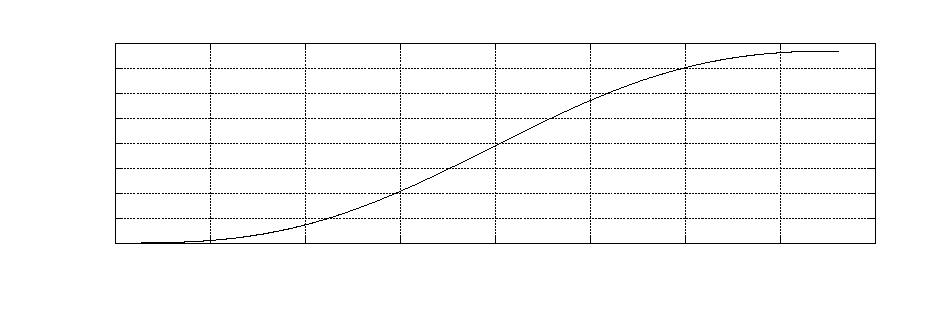
\includegraphics{./sunM}}%
    \gplfronttext
  \end{picture}%
\endgroup

 \end{subfigure} \\
 \begin{subfigure}{\textwidth}
  % GNUPLOT: LaTeX picture with Postscript
\begingroup
  \makeatletter
  \providecommand\color[2][]{%
    \GenericError{(gnuplot) \space\space\space\@spaces}{%
      Package color not loaded in conjunction with
      terminal option `colourtext'%
    }{See the gnuplot documentation for explanation.%
    }{Either use 'blacktext' in gnuplot or load the package
      color.sty in LaTeX.}%
    \renewcommand\color[2][]{}%
  }%
  \providecommand\includegraphics[2][]{%
    \GenericError{(gnuplot) \space\space\space\@spaces}{%
      Package graphicx or graphics not loaded%
    }{See the gnuplot documentation for explanation.%
    }{The gnuplot epslatex terminal needs graphicx.sty or graphics.sty.}%
    \renewcommand\includegraphics[2][]{}%
  }%
  \providecommand\rotatebox[2]{#2}%
  \@ifundefined{ifGPcolor}{%
    \newif\ifGPcolor
    \GPcolortrue
  }{}%
  \@ifundefined{ifGPblacktext}{%
    \newif\ifGPblacktext
    \GPblacktexttrue
  }{}%
  % define a \g@addto@macro without @ in the name:
  \let\gplgaddtomacro\g@addto@macro
  % define empty templates for all commands taking text:
  \gdef\gplbacktext{}%
  \gdef\gplfronttext{}%
  \makeatother
  \ifGPblacktext
    % no textcolor at all
    \def\colorrgb#1{}%
    \def\colorgray#1{}%
  \else
    % gray or color?
    \ifGPcolor
      \def\colorrgb#1{\color[rgb]{#1}}%
      \def\colorgray#1{\color[gray]{#1}}%
      \expandafter\def\csname LTw\endcsname{\color{white}}%
      \expandafter\def\csname LTb\endcsname{\color{black}}%
      \expandafter\def\csname LTa\endcsname{\color{black}}%
      \expandafter\def\csname LT0\endcsname{\color[rgb]{1,0,0}}%
      \expandafter\def\csname LT1\endcsname{\color[rgb]{0,1,0}}%
      \expandafter\def\csname LT2\endcsname{\color[rgb]{0,0,1}}%
      \expandafter\def\csname LT3\endcsname{\color[rgb]{1,0,1}}%
      \expandafter\def\csname LT4\endcsname{\color[rgb]{0,1,1}}%
      \expandafter\def\csname LT5\endcsname{\color[rgb]{1,1,0}}%
      \expandafter\def\csname LT6\endcsname{\color[rgb]{0,0,0}}%
      \expandafter\def\csname LT7\endcsname{\color[rgb]{1,0.3,0}}%
      \expandafter\def\csname LT8\endcsname{\color[rgb]{0.5,0.5,0.5}}%
    \else
      % gray
      \def\colorrgb#1{\color{black}}%
      \def\colorgray#1{\color[gray]{#1}}%
      \expandafter\def\csname LTw\endcsname{\color{white}}%
      \expandafter\def\csname LTb\endcsname{\color{black}}%
      \expandafter\def\csname LTa\endcsname{\color{black}}%
      \expandafter\def\csname LT0\endcsname{\color{black}}%
      \expandafter\def\csname LT1\endcsname{\color{black}}%
      \expandafter\def\csname LT2\endcsname{\color{black}}%
      \expandafter\def\csname LT3\endcsname{\color{black}}%
      \expandafter\def\csname LT4\endcsname{\color{black}}%
      \expandafter\def\csname LT5\endcsname{\color{black}}%
      \expandafter\def\csname LT6\endcsname{\color{black}}%
      \expandafter\def\csname LT7\endcsname{\color{black}}%
      \expandafter\def\csname LT8\endcsname{\color{black}}%
    \fi
  \fi
    \setlength{\unitlength}{0.0500bp}%
    \ifx\gptboxheight\undefined%
      \newlength{\gptboxheight}%
      \newlength{\gptboxwidth}%
      \newsavebox{\gptboxtext}%
    \fi%
    \setlength{\fboxrule}{0.5pt}%
    \setlength{\fboxsep}{1pt}%
\begin{picture}(8640.00,6480.00)%
    \gplgaddtomacro\gplbacktext{%
    }%
    \gplgaddtomacro\gplfronttext{%
      \csname LTb\endcsname%
      \put(176,3459){\rotatebox{-270}{\makebox(0,0){\strut{}$L$ ($L_\odot$)}}}%
      \put(4594,154){\makebox(0,0){\strut{}$r$ ($R_{\odot}$)}}%
      \csname LTb\endcsname%
      \put(814,704){\makebox(0,0)[r]{\strut{}$0$}}%
      \csname LTb\endcsname%
      \put(814,1255){\makebox(0,0)[r]{\strut{}$0.2$}}%
      \csname LTb\endcsname%
      \put(814,1806){\makebox(0,0)[r]{\strut{}$0.4$}}%
      \csname LTb\endcsname%
      \put(814,2357){\makebox(0,0)[r]{\strut{}$0.6$}}%
      \csname LTb\endcsname%
      \put(814,2908){\makebox(0,0)[r]{\strut{}$0.8$}}%
      \csname LTb\endcsname%
      \put(814,3460){\makebox(0,0)[r]{\strut{}$1$}}%
      \csname LTb\endcsname%
      \put(814,4011){\makebox(0,0)[r]{\strut{}$1.2$}}%
      \csname LTb\endcsname%
      \put(814,4562){\makebox(0,0)[r]{\strut{}$1.4$}}%
      \csname LTb\endcsname%
      \put(814,5113){\makebox(0,0)[r]{\strut{}$1.6$}}%
      \csname LTb\endcsname%
      \put(814,5664){\makebox(0,0)[r]{\strut{}$1.8$}}%
      \csname LTb\endcsname%
      \put(814,6215){\makebox(0,0)[r]{\strut{}$2$}}%
      \csname LTb\endcsname%
      \put(946,484){\makebox(0,0){\strut{}$0$}}%
      \csname LTb\endcsname%
      \put(1858,484){\makebox(0,0){\strut{}$0.05$}}%
      \csname LTb\endcsname%
      \put(2770,484){\makebox(0,0){\strut{}$0.1$}}%
      \csname LTb\endcsname%
      \put(3682,484){\makebox(0,0){\strut{}$0.15$}}%
      \csname LTb\endcsname%
      \put(4595,484){\makebox(0,0){\strut{}$0.2$}}%
      \csname LTb\endcsname%
      \put(5507,484){\makebox(0,0){\strut{}$0.25$}}%
      \csname LTb\endcsname%
      \put(6419,484){\makebox(0,0){\strut{}$0.3$}}%
      \csname LTb\endcsname%
      \put(7331,484){\makebox(0,0){\strut{}$0.35$}}%
      \csname LTb\endcsname%
      \put(8243,484){\makebox(0,0){\strut{}$0.4$}}%
    }%
    \gplbacktext
    \put(0,0){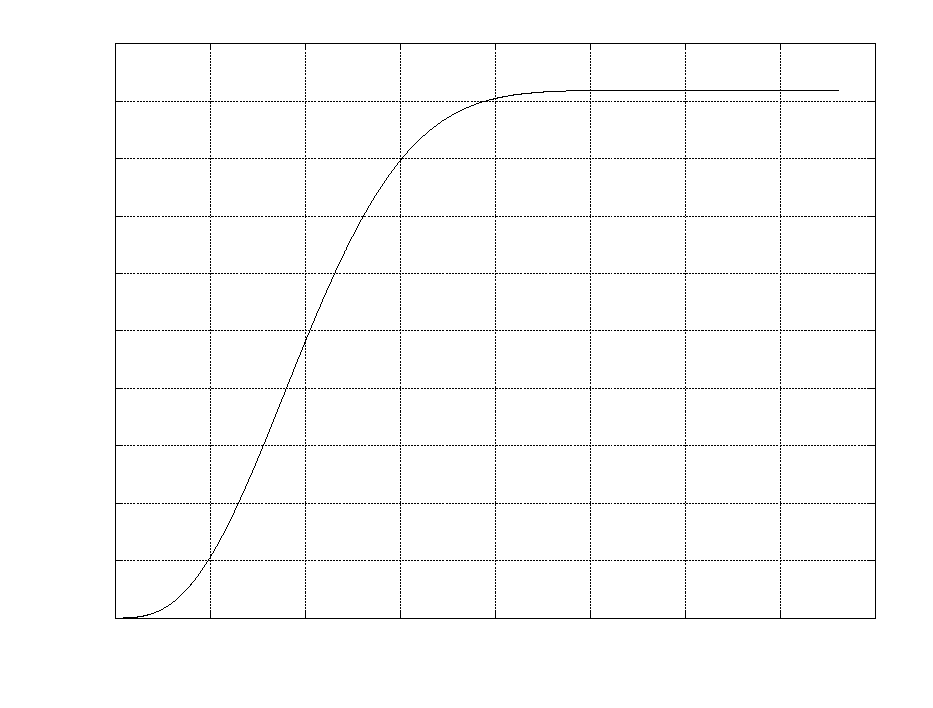
\includegraphics{./sunL}}%
    \gplfronttext
  \end{picture}%
\endgroup

 \end{subfigure} \\
  \begin{subfigure}{\textwidth}
  % GNUPLOT: LaTeX picture with Postscript
\begingroup
  \makeatletter
  \providecommand\color[2][]{%
    \GenericError{(gnuplot) \space\space\space\@spaces}{%
      Package color not loaded in conjunction with
      terminal option `colourtext'%
    }{See the gnuplot documentation for explanation.%
    }{Either use 'blacktext' in gnuplot or load the package
      color.sty in LaTeX.}%
    \renewcommand\color[2][]{}%
  }%
  \providecommand\includegraphics[2][]{%
    \GenericError{(gnuplot) \space\space\space\@spaces}{%
      Package graphicx or graphics not loaded%
    }{See the gnuplot documentation for explanation.%
    }{The gnuplot epslatex terminal needs graphicx.sty or graphics.sty.}%
    \renewcommand\includegraphics[2][]{}%
  }%
  \providecommand\rotatebox[2]{#2}%
  \@ifundefined{ifGPcolor}{%
    \newif\ifGPcolor
    \GPcolortrue
  }{}%
  \@ifundefined{ifGPblacktext}{%
    \newif\ifGPblacktext
    \GPblacktexttrue
  }{}%
  % define a \g@addto@macro without @ in the name:
  \let\gplgaddtomacro\g@addto@macro
  % define empty templates for all commands taking text:
  \gdef\gplbacktext{}%
  \gdef\gplfronttext{}%
  \makeatother
  \ifGPblacktext
    % no textcolor at all
    \def\colorrgb#1{}%
    \def\colorgray#1{}%
  \else
    % gray or color?
    \ifGPcolor
      \def\colorrgb#1{\color[rgb]{#1}}%
      \def\colorgray#1{\color[gray]{#1}}%
      \expandafter\def\csname LTw\endcsname{\color{white}}%
      \expandafter\def\csname LTb\endcsname{\color{black}}%
      \expandafter\def\csname LTa\endcsname{\color{black}}%
      \expandafter\def\csname LT0\endcsname{\color[rgb]{1,0,0}}%
      \expandafter\def\csname LT1\endcsname{\color[rgb]{0,1,0}}%
      \expandafter\def\csname LT2\endcsname{\color[rgb]{0,0,1}}%
      \expandafter\def\csname LT3\endcsname{\color[rgb]{1,0,1}}%
      \expandafter\def\csname LT4\endcsname{\color[rgb]{0,1,1}}%
      \expandafter\def\csname LT5\endcsname{\color[rgb]{1,1,0}}%
      \expandafter\def\csname LT6\endcsname{\color[rgb]{0,0,0}}%
      \expandafter\def\csname LT7\endcsname{\color[rgb]{1,0.3,0}}%
      \expandafter\def\csname LT8\endcsname{\color[rgb]{0.5,0.5,0.5}}%
    \else
      % gray
      \def\colorrgb#1{\color{black}}%
      \def\colorgray#1{\color[gray]{#1}}%
      \expandafter\def\csname LTw\endcsname{\color{white}}%
      \expandafter\def\csname LTb\endcsname{\color{black}}%
      \expandafter\def\csname LTa\endcsname{\color{black}}%
      \expandafter\def\csname LT0\endcsname{\color{black}}%
      \expandafter\def\csname LT1\endcsname{\color{black}}%
      \expandafter\def\csname LT2\endcsname{\color{black}}%
      \expandafter\def\csname LT3\endcsname{\color{black}}%
      \expandafter\def\csname LT4\endcsname{\color{black}}%
      \expandafter\def\csname LT5\endcsname{\color{black}}%
      \expandafter\def\csname LT6\endcsname{\color{black}}%
      \expandafter\def\csname LT7\endcsname{\color{black}}%
      \expandafter\def\csname LT8\endcsname{\color{black}}%
    \fi
  \fi
    \setlength{\unitlength}{0.0500bp}%
    \ifx\gptboxheight\undefined%
      \newlength{\gptboxheight}%
      \newlength{\gptboxwidth}%
      \newsavebox{\gptboxtext}%
    \fi%
    \setlength{\fboxrule}{0.5pt}%
    \setlength{\fboxsep}{1pt}%
\begin{picture}(8640.00,2880.00)%
    \gplgaddtomacro\gplbacktext{%
    }%
    \gplgaddtomacro\gplfronttext{%
      \csname LTb\endcsname%
      \put(176,1659){\rotatebox{-270}{\makebox(0,0){\strut{}$T$ (K)}}}%
      \put(4858,154){\makebox(0,0){\strut{}$r$ ($R_{\odot}$)}}%
      \csname LTb\endcsname%
      \put(1342,704){\makebox(0,0)[r]{\strut{}$0$}}%
      \csname LTb\endcsname%
      \put(1342,943){\makebox(0,0)[r]{\strut{}$2\times10^{6}$}}%
      \csname LTb\endcsname%
      \put(1342,1182){\makebox(0,0)[r]{\strut{}$4\times10^{6}$}}%
      \csname LTb\endcsname%
      \put(1342,1421){\makebox(0,0)[r]{\strut{}$6\times10^{6}$}}%
      \csname LTb\endcsname%
      \put(1342,1660){\makebox(0,0)[r]{\strut{}$8\times10^{6}$}}%
      \csname LTb\endcsname%
      \put(1342,1898){\makebox(0,0)[r]{\strut{}$1\times10^{7}$}}%
      \csname LTb\endcsname%
      \put(1342,2137){\makebox(0,0)[r]{\strut{}$1.2\times10^{7}$}}%
      \csname LTb\endcsname%
      \put(1342,2376){\makebox(0,0)[r]{\strut{}$1.4\times10^{7}$}}%
      \csname LTb\endcsname%
      \put(1342,2615){\makebox(0,0)[r]{\strut{}$1.6\times10^{7}$}}%
      \csname LTb\endcsname%
      \put(1474,484){\makebox(0,0){\strut{}$0$}}%
      \csname LTb\endcsname%
      \put(2320,484){\makebox(0,0){\strut{}$0.05$}}%
      \csname LTb\endcsname%
      \put(3166,484){\makebox(0,0){\strut{}$0.1$}}%
      \csname LTb\endcsname%
      \put(4012,484){\makebox(0,0){\strut{}$0.15$}}%
      \csname LTb\endcsname%
      \put(4859,484){\makebox(0,0){\strut{}$0.2$}}%
      \csname LTb\endcsname%
      \put(5705,484){\makebox(0,0){\strut{}$0.25$}}%
      \csname LTb\endcsname%
      \put(6551,484){\makebox(0,0){\strut{}$0.3$}}%
      \csname LTb\endcsname%
      \put(7397,484){\makebox(0,0){\strut{}$0.35$}}%
      \csname LTb\endcsname%
      \put(8243,484){\makebox(0,0){\strut{}$0.4$}}%
    }%
    \gplbacktext
    \put(0,0){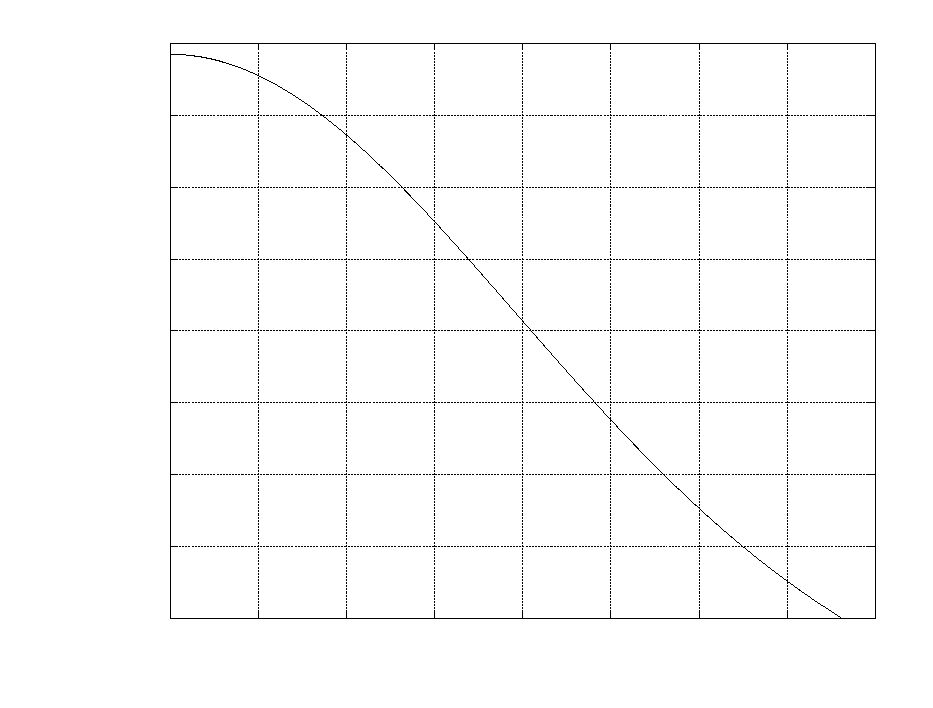
\includegraphics{./sunT}}%
    \gplfronttext
  \end{picture}%
\endgroup

 \end{subfigure} \\
   \begin{subfigure}{\textwidth}
  % GNUPLOT: LaTeX picture with Postscript
\begingroup
  \makeatletter
  \providecommand\color[2][]{%
    \GenericError{(gnuplot) \space\space\space\@spaces}{%
      Package color not loaded in conjunction with
      terminal option `colourtext'%
    }{See the gnuplot documentation for explanation.%
    }{Either use 'blacktext' in gnuplot or load the package
      color.sty in LaTeX.}%
    \renewcommand\color[2][]{}%
  }%
  \providecommand\includegraphics[2][]{%
    \GenericError{(gnuplot) \space\space\space\@spaces}{%
      Package graphicx or graphics not loaded%
    }{See the gnuplot documentation for explanation.%
    }{The gnuplot epslatex terminal needs graphicx.sty or graphics.sty.}%
    \renewcommand\includegraphics[2][]{}%
  }%
  \providecommand\rotatebox[2]{#2}%
  \@ifundefined{ifGPcolor}{%
    \newif\ifGPcolor
    \GPcolortrue
  }{}%
  \@ifundefined{ifGPblacktext}{%
    \newif\ifGPblacktext
    \GPblacktexttrue
  }{}%
  % define a \g@addto@macro without @ in the name:
  \let\gplgaddtomacro\g@addto@macro
  % define empty templates for all commands taking text:
  \gdef\gplbacktext{}%
  \gdef\gplfronttext{}%
  \makeatother
  \ifGPblacktext
    % no textcolor at all
    \def\colorrgb#1{}%
    \def\colorgray#1{}%
  \else
    % gray or color?
    \ifGPcolor
      \def\colorrgb#1{\color[rgb]{#1}}%
      \def\colorgray#1{\color[gray]{#1}}%
      \expandafter\def\csname LTw\endcsname{\color{white}}%
      \expandafter\def\csname LTb\endcsname{\color{black}}%
      \expandafter\def\csname LTa\endcsname{\color{black}}%
      \expandafter\def\csname LT0\endcsname{\color[rgb]{1,0,0}}%
      \expandafter\def\csname LT1\endcsname{\color[rgb]{0,1,0}}%
      \expandafter\def\csname LT2\endcsname{\color[rgb]{0,0,1}}%
      \expandafter\def\csname LT3\endcsname{\color[rgb]{1,0,1}}%
      \expandafter\def\csname LT4\endcsname{\color[rgb]{0,1,1}}%
      \expandafter\def\csname LT5\endcsname{\color[rgb]{1,1,0}}%
      \expandafter\def\csname LT6\endcsname{\color[rgb]{0,0,0}}%
      \expandafter\def\csname LT7\endcsname{\color[rgb]{1,0.3,0}}%
      \expandafter\def\csname LT8\endcsname{\color[rgb]{0.5,0.5,0.5}}%
    \else
      % gray
      \def\colorrgb#1{\color{black}}%
      \def\colorgray#1{\color[gray]{#1}}%
      \expandafter\def\csname LTw\endcsname{\color{white}}%
      \expandafter\def\csname LTb\endcsname{\color{black}}%
      \expandafter\def\csname LTa\endcsname{\color{black}}%
      \expandafter\def\csname LT0\endcsname{\color{black}}%
      \expandafter\def\csname LT1\endcsname{\color{black}}%
      \expandafter\def\csname LT2\endcsname{\color{black}}%
      \expandafter\def\csname LT3\endcsname{\color{black}}%
      \expandafter\def\csname LT4\endcsname{\color{black}}%
      \expandafter\def\csname LT5\endcsname{\color{black}}%
      \expandafter\def\csname LT6\endcsname{\color{black}}%
      \expandafter\def\csname LT7\endcsname{\color{black}}%
      \expandafter\def\csname LT8\endcsname{\color{black}}%
    \fi
  \fi
    \setlength{\unitlength}{0.0500bp}%
    \ifx\gptboxheight\undefined%
      \newlength{\gptboxheight}%
      \newlength{\gptboxwidth}%
      \newsavebox{\gptboxtext}%
    \fi%
    \setlength{\fboxrule}{0.5pt}%
    \setlength{\fboxsep}{1pt}%
\begin{picture}(8640.00,2880.00)%
    \gplgaddtomacro\gplbacktext{%
    }%
    \gplgaddtomacro\gplfronttext{%
      \csname LTb\endcsname%
      \put(176,1659){\rotatebox{-270}{\makebox(0,0){\strut{}$P$ (Pa)}}}%
      \put(4924,154){\makebox(0,0){\strut{}$r$ ($R_{\odot}$)}}%
      \csname LTb\endcsname%
      \put(1474,704){\makebox(0,0)[r]{\strut{}$0$}}%
      \csname LTb\endcsname%
      \put(1474,1086){\makebox(0,0)[r]{\strut{}$5\times10^{15}$}}%
      \csname LTb\endcsname%
      \put(1474,1468){\makebox(0,0)[r]{\strut{}$1\times10^{16}$}}%
      \csname LTb\endcsname%
      \put(1474,1851){\makebox(0,0)[r]{\strut{}$1.5\times10^{16}$}}%
      \csname LTb\endcsname%
      \put(1474,2233){\makebox(0,0)[r]{\strut{}$2\times10^{16}$}}%
      \csname LTb\endcsname%
      \put(1474,2615){\makebox(0,0)[r]{\strut{}$2.5\times10^{16}$}}%
      \csname LTb\endcsname%
      \put(1606,484){\makebox(0,0){\strut{}$0$}}%
      \csname LTb\endcsname%
      \put(2436,484){\makebox(0,0){\strut{}$0.05$}}%
      \csname LTb\endcsname%
      \put(3265,484){\makebox(0,0){\strut{}$0.1$}}%
      \csname LTb\endcsname%
      \put(4095,484){\makebox(0,0){\strut{}$0.15$}}%
      \csname LTb\endcsname%
      \put(4925,484){\makebox(0,0){\strut{}$0.2$}}%
      \csname LTb\endcsname%
      \put(5754,484){\makebox(0,0){\strut{}$0.25$}}%
      \csname LTb\endcsname%
      \put(6584,484){\makebox(0,0){\strut{}$0.3$}}%
      \csname LTb\endcsname%
      \put(7413,484){\makebox(0,0){\strut{}$0.35$}}%
      \csname LTb\endcsname%
      \put(8243,484){\makebox(0,0){\strut{}$0.4$}}%
    }%
    \gplbacktext
    \put(0,0){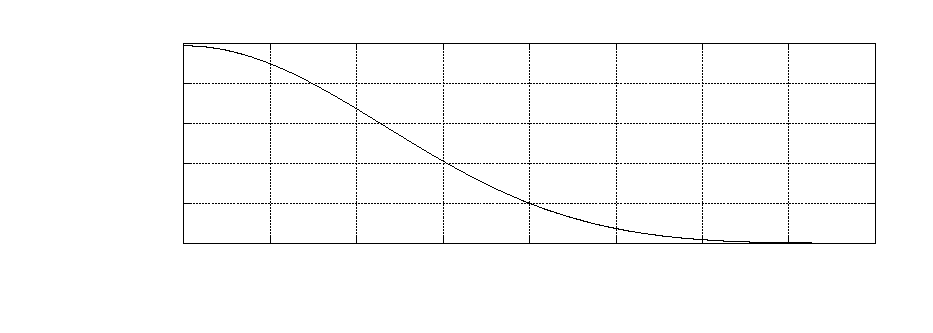
\includegraphics{./sunP}}%
    \gplfronttext
  \end{picture}%
\endgroup

 \end{subfigure}
 \caption{Simulation results of the Sun.}
 \label{fig:sun}
 \end{centering}
\end{figure}

\section{Results}
Figure \ref{fig:sun} shows our results using the initial conditions of the core of the sun. These plots have the general trend we would expect for a 1 solar mass star, but they do not get the exact final values of the sun. One thing that differs from our star to the sun is that it is only radiative for two radius steps, which is about $2\times 10^5$ meters, and convective for the rest. This is in contrast to the sun, where the radiative zone is about 70\% of the whole star. Because of this, the boundary conditions were not met perfectly; the surface temperature should go to zero but our pressure hit zero first, triggering the integration to stop every time. The mass of our star was about 0.78 $M_\odot$, it's radius was only around 0.38 $R_\odot$, which is considerably smaller. The luminosity was about 1.8 $ L_\odot$. If the model was perfect, we would expect the final values for mass, luminosity, temperature, and pressure to be approximately $1 M_\odot$, $1 L_\odot$, $5770$ K, and $0$ Pa, respectively. \\

Knowing our model works generally, but is not perfect, we go forwards to use it on other stars and get a general form of the main sequence of an HR diagram. Now, an HR diagram is a log plot of the luminosity vs. effective temperature. The effective temperature is observationally found by matching the color of a star to temperature that emits that color the most. Because of this, it is not the surface temperature, rather, the temperature from an optical depth inside the star. Our attempts to calculate the optical depths of our stars resulted in wildly large values that were thousands of times larger than the star itself. However, because during our integrations the pressure was going to zero, a convenient to use surface temperature remains. This is not perfect, but should still give us a good relationship between different stars temperatures. Our first attempt at an HR diagram used all of the raw data and is shown in Figure \ref{fig:badHR}. \\

The first obvious thing that you'll notice is that the stars seem to have four distinct categories. A small group with high temperatures and luminosities, two groups with low temperatures and luminosities, and a large group somewhere in the middle. To help make some sense of whatw as going on, we then included the radii of the stars on a new plot, shown in Figure \ref{fig:nosobadHR}. \\

We can see that the shape resembles the main sequence part of the known HR diagram. We can explore a well known program to get a sense of what the HR diagram should look like and compare it to our own model. We will use MESA to do the comparison. MESA will give us a plot of the total life of a star. We can compare where our model shows the stars on the main sequence and we expect the MESA star to be on the main sequence at some point in its life. MESA considers different characteristics that  we do not consider in our model. Our model is static, has no rotation and it is only for main sequence stars and MESA will allow for rotation and it does a full life of a star so it is not static and will not only be on the main sequence. \\ 

The main goal was to create an HR diagram by simulating a star manually and plotting the data. To do this we needed to complete many sub-parts along the way. The first objective of our team was to get a profile on github and ensure everyone knows how to pull, add, commit and push properly. In the first few tries there were of course a couple troubles where someone forgot to pull right before pushing to ensure their version was up to date with the original. Eventually, everyone was able to pull, add, commit then push a change with no problems. Splitting up work in a fair and convenient way was a small challenge. Working in a big group makes it easier to write the code because we are able to all bring our ideas together and come up with a solution faster. We learned to work as a group in an efficient way, even though our ideas would not work sometimes we were able to listen to everyone and everyone was able to contribute. Different people have different styles of writing code so working in a group of five each person has to learn to read and interpret someone elses code. At the same time, we learned to comment our code so that the rest of our group would be able to understand what had been written and why.\\


\begin{figure}[p]
\begin{centering}
% GNUPLOT: LaTeX picture with Postscript
\begingroup
  \makeatletter
  \providecommand\color[2][]{%
    \GenericError{(gnuplot) \space\space\space\@spaces}{%
      Package color not loaded in conjunction with
      terminal option `colourtext'%
    }{See the gnuplot documentation for explanation.%
    }{Either use 'blacktext' in gnuplot or load the package
      color.sty in LaTeX.}%
    \renewcommand\color[2][]{}%
  }%
  \providecommand\includegraphics[2][]{%
    \GenericError{(gnuplot) \space\space\space\@spaces}{%
      Package graphicx or graphics not loaded%
    }{See the gnuplot documentation for explanation.%
    }{The gnuplot epslatex terminal needs graphicx.sty or graphics.sty.}%
    \renewcommand\includegraphics[2][]{}%
  }%
  \providecommand\rotatebox[2]{#2}%
  \@ifundefined{ifGPcolor}{%
    \newif\ifGPcolor
    \GPcolortrue
  }{}%
  \@ifundefined{ifGPblacktext}{%
    \newif\ifGPblacktext
    \GPblacktexttrue
  }{}%
  % define a \g@addto@macro without @ in the name:
  \let\gplgaddtomacro\g@addto@macro
  % define empty templates for all commands taking text:
  \gdef\gplbacktext{}%
  \gdef\gplfronttext{}%
  \makeatother
  \ifGPblacktext
    % no textcolor at all
    \def\colorrgb#1{}%
    \def\colorgray#1{}%
  \else
    % gray or color?
    \ifGPcolor
      \def\colorrgb#1{\color[rgb]{#1}}%
      \def\colorgray#1{\color[gray]{#1}}%
      \expandafter\def\csname LTw\endcsname{\color{white}}%
      \expandafter\def\csname LTb\endcsname{\color{black}}%
      \expandafter\def\csname LTa\endcsname{\color{black}}%
      \expandafter\def\csname LT0\endcsname{\color[rgb]{1,0,0}}%
      \expandafter\def\csname LT1\endcsname{\color[rgb]{0,1,0}}%
      \expandafter\def\csname LT2\endcsname{\color[rgb]{0,0,1}}%
      \expandafter\def\csname LT3\endcsname{\color[rgb]{1,0,1}}%
      \expandafter\def\csname LT4\endcsname{\color[rgb]{0,1,1}}%
      \expandafter\def\csname LT5\endcsname{\color[rgb]{1,1,0}}%
      \expandafter\def\csname LT6\endcsname{\color[rgb]{0,0,0}}%
      \expandafter\def\csname LT7\endcsname{\color[rgb]{1,0.3,0}}%
      \expandafter\def\csname LT8\endcsname{\color[rgb]{0.5,0.5,0.5}}%
    \else
      % gray
      \def\colorrgb#1{\color{black}}%
      \def\colorgray#1{\color[gray]{#1}}%
      \expandafter\def\csname LTw\endcsname{\color{white}}%
      \expandafter\def\csname LTb\endcsname{\color{black}}%
      \expandafter\def\csname LTa\endcsname{\color{black}}%
      \expandafter\def\csname LT0\endcsname{\color{black}}%
      \expandafter\def\csname LT1\endcsname{\color{black}}%
      \expandafter\def\csname LT2\endcsname{\color{black}}%
      \expandafter\def\csname LT3\endcsname{\color{black}}%
      \expandafter\def\csname LT4\endcsname{\color{black}}%
      \expandafter\def\csname LT5\endcsname{\color{black}}%
      \expandafter\def\csname LT6\endcsname{\color{black}}%
      \expandafter\def\csname LT7\endcsname{\color{black}}%
      \expandafter\def\csname LT8\endcsname{\color{black}}%
    \fi
  \fi
    \setlength{\unitlength}{0.0500bp}%
    \ifx\gptboxheight\undefined%
      \newlength{\gptboxheight}%
      \newlength{\gptboxwidth}%
      \newsavebox{\gptboxtext}%
    \fi%
    \setlength{\fboxrule}{0.5pt}%
    \setlength{\fboxsep}{1pt}%
\begin{picture}(8640.00,6480.00)%
    \gplgaddtomacro\gplbacktext{%
    }%
    \gplgaddtomacro\gplfronttext{%
      \csname LTb\endcsname%
      \put(176,3459){\rotatebox{-270}{\makebox(0,0){\strut{}$L$ ($L_\odot$)}}}%
      \put(4726,154){\makebox(0,0){\strut{}$T$ (K)}}%
      \csname LTb\endcsname%
      \put(1078,704){\makebox(0,0)[r]{\strut{}$10^{-35}$}}%
      \csname LTb\endcsname%
      \put(1078,1205){\makebox(0,0)[r]{\strut{}$10^{-30}$}}%
      \csname LTb\endcsname%
      \put(1078,1706){\makebox(0,0)[r]{\strut{}$10^{-25}$}}%
      \csname LTb\endcsname%
      \put(1078,2207){\makebox(0,0)[r]{\strut{}$10^{-20}$}}%
      \csname LTb\endcsname%
      \put(1078,2708){\makebox(0,0)[r]{\strut{}$10^{-15}$}}%
      \csname LTb\endcsname%
      \put(1078,3209){\makebox(0,0)[r]{\strut{}$10^{-10}$}}%
      \csname LTb\endcsname%
      \put(1078,3710){\makebox(0,0)[r]{\strut{}$10^{-5}$}}%
      \csname LTb\endcsname%
      \put(1078,4211){\makebox(0,0)[r]{\strut{}$10^{0}$}}%
      \csname LTb\endcsname%
      \put(1078,4712){\makebox(0,0)[r]{\strut{}$10^{5}$}}%
      \csname LTb\endcsname%
      \put(1078,5213){\makebox(0,0)[r]{\strut{}$10^{10}$}}%
      \csname LTb\endcsname%
      \put(1078,5714){\makebox(0,0)[r]{\strut{}$10^{15}$}}%
      \csname LTb\endcsname%
      \put(1078,6215){\makebox(0,0)[r]{\strut{}$10^{20}$}}%
      \csname LTb\endcsname%
      \put(8243,484){\makebox(0,0){\strut{}$10^{1}$}}%
      \csname LTb\endcsname%
      \put(7462,484){\makebox(0,0){\strut{}$10^{2}$}}%
      \csname LTb\endcsname%
      \put(6680,484){\makebox(0,0){\strut{}$10^{3}$}}%
      \csname LTb\endcsname%
      \put(5899,484){\makebox(0,0){\strut{}$10^{4}$}}%
      \csname LTb\endcsname%
      \put(5117,484){\makebox(0,0){\strut{}$10^{5}$}}%
      \csname LTb\endcsname%
      \put(4336,484){\makebox(0,0){\strut{}$10^{6}$}}%
      \csname LTb\endcsname%
      \put(3554,484){\makebox(0,0){\strut{}$10^{7}$}}%
      \csname LTb\endcsname%
      \put(2773,484){\makebox(0,0){\strut{}$10^{8}$}}%
      \csname LTb\endcsname%
      \put(1991,484){\makebox(0,0){\strut{}$10^{9}$}}%
      \csname LTb\endcsname%
      \put(1210,484){\makebox(0,0){\strut{}$10^{10}$}}%
    }%
    \gplbacktext
    \put(0,0){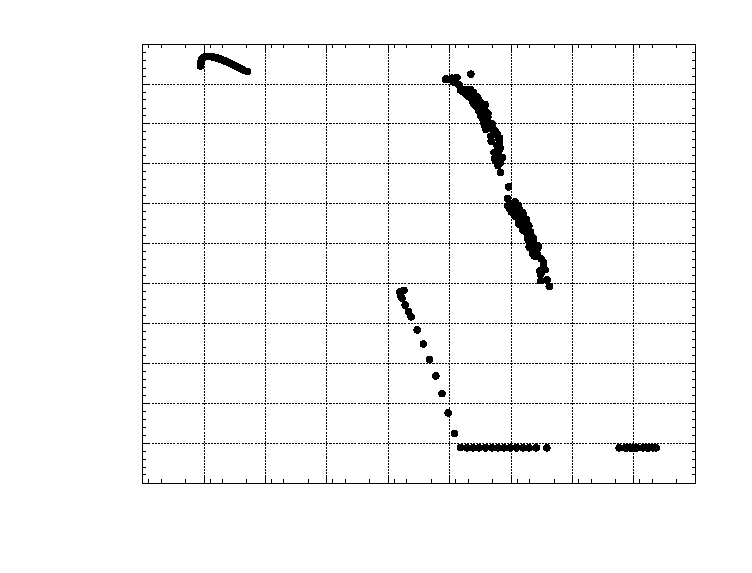
\includegraphics{./badHR}}%
    \gplfronttext
  \end{picture}%
\endgroup

\caption{A crappy version of HR}
\label{fig:badHR}
\end{centering}
\end{figure}

\begin{figure}[p]
\begin{centering}
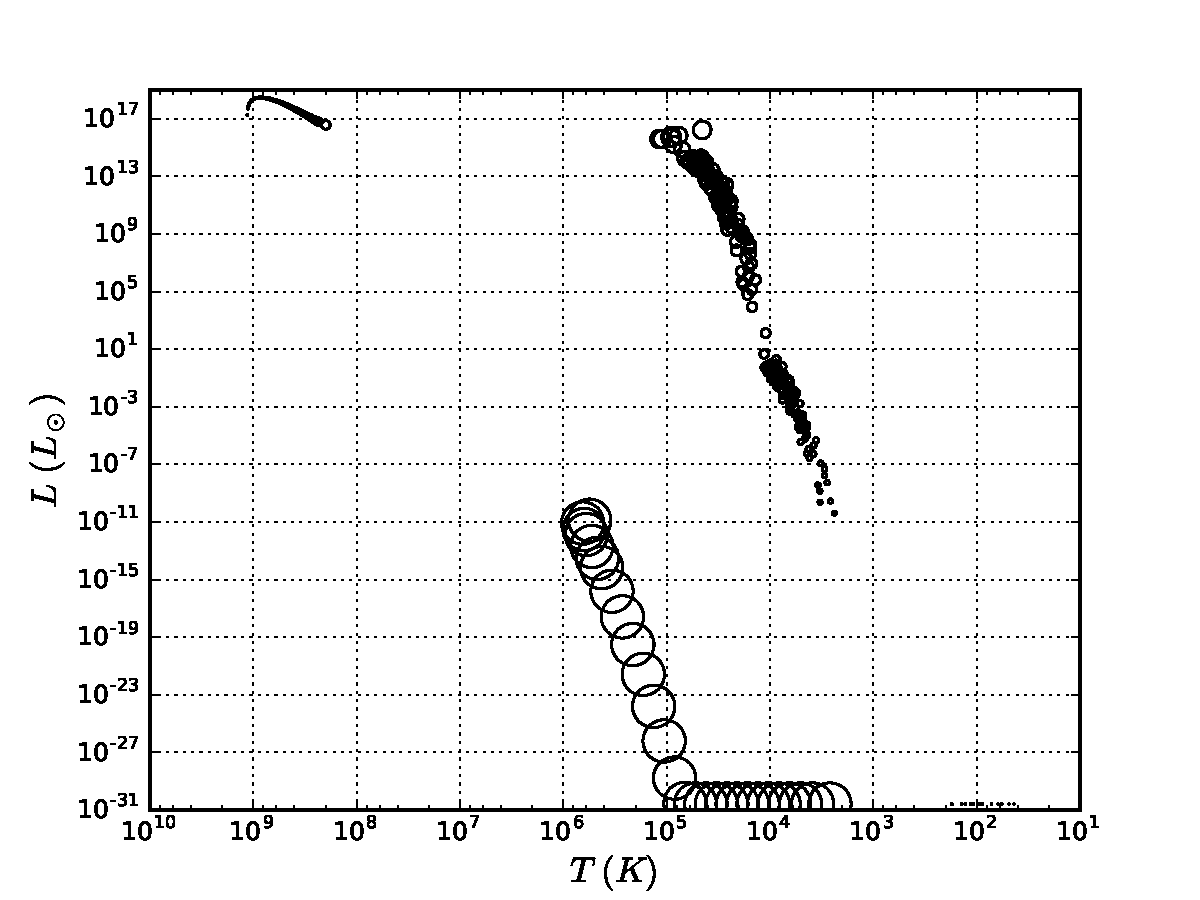
\includegraphics[width=\textwidth]{new_bad_hr.pdf}
\caption{A crappy version of HR}
\label{fig:nosobadHR}
\end{centering}
\end{figure}

\begin{figure}[p]
\begin{centering}
% GNUPLOT: LaTeX picture with Postscript
\begingroup
  \makeatletter
  \providecommand\color[2][]{%
    \GenericError{(gnuplot) \space\space\space\@spaces}{%
      Package color not loaded in conjunction with
      terminal option `colourtext'%
    }{See the gnuplot documentation for explanation.%
    }{Either use 'blacktext' in gnuplot or load the package
      color.sty in LaTeX.}%
    \renewcommand\color[2][]{}%
  }%
  \providecommand\includegraphics[2][]{%
    \GenericError{(gnuplot) \space\space\space\@spaces}{%
      Package graphicx or graphics not loaded%
    }{See the gnuplot documentation for explanation.%
    }{The gnuplot epslatex terminal needs graphicx.sty or graphics.sty.}%
    \renewcommand\includegraphics[2][]{}%
  }%
  \providecommand\rotatebox[2]{#2}%
  \@ifundefined{ifGPcolor}{%
    \newif\ifGPcolor
    \GPcolortrue
  }{}%
  \@ifundefined{ifGPblacktext}{%
    \newif\ifGPblacktext
    \GPblacktexttrue
  }{}%
  % define a \g@addto@macro without @ in the name:
  \let\gplgaddtomacro\g@addto@macro
  % define empty templates for all commands taking text:
  \gdef\gplbacktext{}%
  \gdef\gplfronttext{}%
  \makeatother
  \ifGPblacktext
    % no textcolor at all
    \def\colorrgb#1{}%
    \def\colorgray#1{}%
  \else
    % gray or color?
    \ifGPcolor
      \def\colorrgb#1{\color[rgb]{#1}}%
      \def\colorgray#1{\color[gray]{#1}}%
      \expandafter\def\csname LTw\endcsname{\color{white}}%
      \expandafter\def\csname LTb\endcsname{\color{black}}%
      \expandafter\def\csname LTa\endcsname{\color{black}}%
      \expandafter\def\csname LT0\endcsname{\color[rgb]{1,0,0}}%
      \expandafter\def\csname LT1\endcsname{\color[rgb]{0,1,0}}%
      \expandafter\def\csname LT2\endcsname{\color[rgb]{0,0,1}}%
      \expandafter\def\csname LT3\endcsname{\color[rgb]{1,0,1}}%
      \expandafter\def\csname LT4\endcsname{\color[rgb]{0,1,1}}%
      \expandafter\def\csname LT5\endcsname{\color[rgb]{1,1,0}}%
      \expandafter\def\csname LT6\endcsname{\color[rgb]{0,0,0}}%
      \expandafter\def\csname LT7\endcsname{\color[rgb]{1,0.3,0}}%
      \expandafter\def\csname LT8\endcsname{\color[rgb]{0.5,0.5,0.5}}%
    \else
      % gray
      \def\colorrgb#1{\color{black}}%
      \def\colorgray#1{\color[gray]{#1}}%
      \expandafter\def\csname LTw\endcsname{\color{white}}%
      \expandafter\def\csname LTb\endcsname{\color{black}}%
      \expandafter\def\csname LTa\endcsname{\color{black}}%
      \expandafter\def\csname LT0\endcsname{\color{black}}%
      \expandafter\def\csname LT1\endcsname{\color{black}}%
      \expandafter\def\csname LT2\endcsname{\color{black}}%
      \expandafter\def\csname LT3\endcsname{\color{black}}%
      \expandafter\def\csname LT4\endcsname{\color{black}}%
      \expandafter\def\csname LT5\endcsname{\color{black}}%
      \expandafter\def\csname LT6\endcsname{\color{black}}%
      \expandafter\def\csname LT7\endcsname{\color{black}}%
      \expandafter\def\csname LT8\endcsname{\color{black}}%
    \fi
  \fi
    \setlength{\unitlength}{0.0500bp}%
    \ifx\gptboxheight\undefined%
      \newlength{\gptboxheight}%
      \newlength{\gptboxwidth}%
      \newsavebox{\gptboxtext}%
    \fi%
    \setlength{\fboxrule}{0.5pt}%
    \setlength{\fboxsep}{1pt}%
\begin{picture}(8640.00,6480.00)%
    \gplgaddtomacro\gplbacktext{%
    }%
    \gplgaddtomacro\gplfronttext{%
      \csname LTb\endcsname%
      \put(176,3899){\rotatebox{-270}{\makebox(0,0){\strut{}$L$ ($L_\odot$)}}}%
      \put(4726,1034){\makebox(0,0){\strut{}$T$ (K)}}%
      \csname LTb\endcsname%
      \put(3871,833){\makebox(0,0)[r]{\strut{}MESA star}}%
      \csname LTb\endcsname%
      \put(3871,613){\makebox(0,0)[r]{\strut{}MESA star}}%
      \csname LTb\endcsname%
      \put(3871,393){\makebox(0,0)[r]{\strut{}MESA star}}%
      \csname LTb\endcsname%
      \put(3871,173){\makebox(0,0)[r]{\strut{}MESA star}}%
      \csname LTb\endcsname%
      \put(6706,833){\makebox(0,0)[r]{\strut{}MESA star}}%
      \csname LTb\endcsname%
      \put(6706,613){\makebox(0,0)[r]{\strut{}Real Stars}}%
      \csname LTb\endcsname%
      \put(6706,393){\makebox(0,0)[r]{\strut{}Simulated Stars}}%
      \csname LTb\endcsname%
      \put(1078,1584){\makebox(0,0)[r]{\strut{}$10^{-12}$}}%
      \csname LTb\endcsname%
      \put(1078,2047){\makebox(0,0)[r]{\strut{}$10^{-10}$}}%
      \csname LTb\endcsname%
      \put(1078,2510){\makebox(0,0)[r]{\strut{}$10^{-8}$}}%
      \csname LTb\endcsname%
      \put(1078,2973){\makebox(0,0)[r]{\strut{}$10^{-6}$}}%
      \csname LTb\endcsname%
      \put(1078,3436){\makebox(0,0)[r]{\strut{}$10^{-4}$}}%
      \csname LTb\endcsname%
      \put(1078,3900){\makebox(0,0)[r]{\strut{}$10^{-2}$}}%
      \csname LTb\endcsname%
      \put(1078,4363){\makebox(0,0)[r]{\strut{}$10^{0}$}}%
      \csname LTb\endcsname%
      \put(1078,4826){\makebox(0,0)[r]{\strut{}$10^{2}$}}%
      \csname LTb\endcsname%
      \put(1078,5289){\makebox(0,0)[r]{\strut{}$10^{4}$}}%
      \csname LTb\endcsname%
      \put(1078,5752){\makebox(0,0)[r]{\strut{}$10^{6}$}}%
      \csname LTb\endcsname%
      \put(1078,6215){\makebox(0,0)[r]{\strut{}$10^{8}$}}%
      \csname LTb\endcsname%
      \put(8243,1364){\makebox(0,0){\strut{}$10^{3}$}}%
      \csname LTb\endcsname%
      \put(4727,1364){\makebox(0,0){\strut{}$10^{4}$}}%
      \csname LTb\endcsname%
      \put(1210,1364){\makebox(0,0){\strut{}$10^{5}$}}%
    }%
    \gplbacktext
    \put(0,0){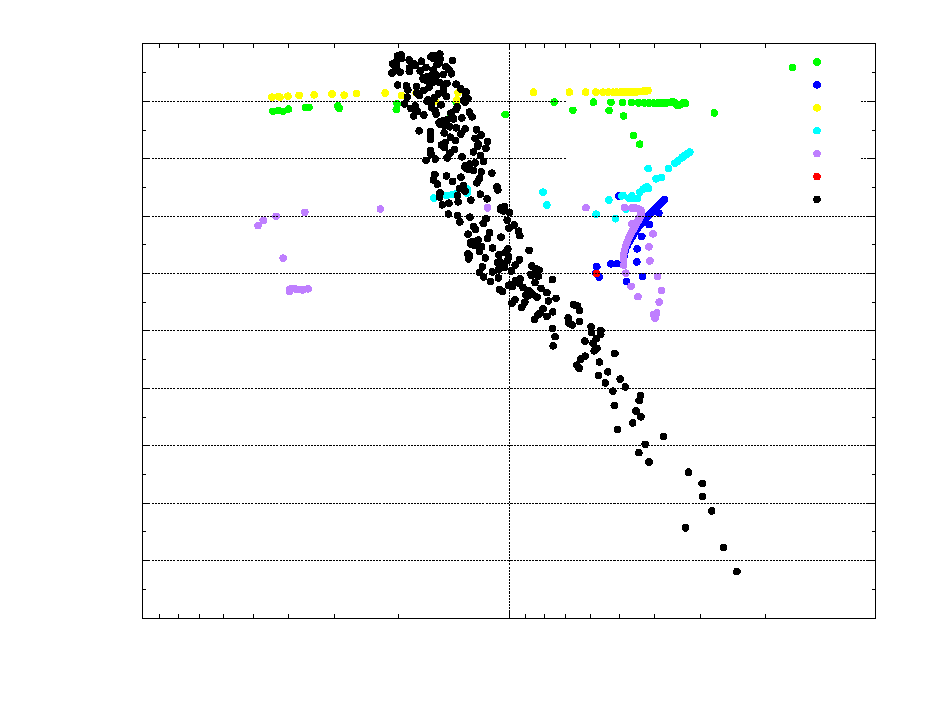
\includegraphics{./HR}}%
    \gplfronttext
  \end{picture}%
\endgroup

\caption{Our reproduction of the HR diagram.}
\label{fig:HR}
\end{centering}
\end{figure}

\begin{figure}[p]
\begin{centering}
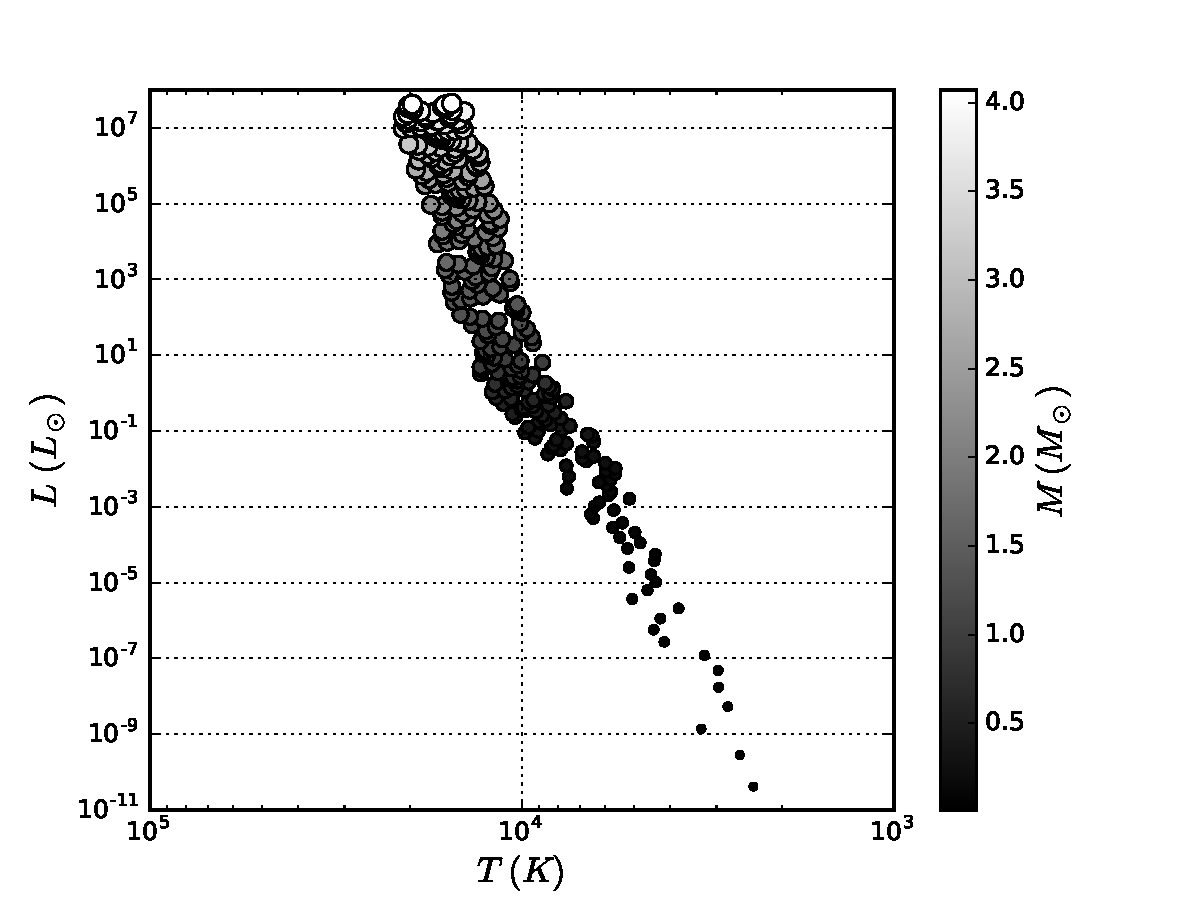
\includegraphics[width=\textwidth]{extra_hr.pdf}
\caption{Another perspective on our HR}
\label{fig:extraHR}
\end{centering}
\end{figure}


\end{document}
